\documentclass{beamer}

\usepackage{tikz}
\usepackage[progressbar=foot]{theme/beamerthememetropolis}

\setbeamercovered{transparent}
\usetikzlibrary{overlay-beamer-styles}
\tikzset{
    highlight on/.style={alt={#1{fill=red!80!black,color=red!80!black}{fill=gray!30!white,color=gray!30!white}}},
}

\iffalse
I'm a chromium engineer who's responsible for launching HLS playback natively in the chromium project (and thus the Google Chrome browser).

The talk I plan to give starts by including a brief overview of the history of HLS in browsers, including how we got to the point of launching it in Chrome.

Next up is an explanation of how this new player works, and what advantages we can make use of by building it into the browser vs shipping packaged javascript. I haven't yet decided how technical I will get when talking about the chromium pipeline/demuxer/decoder architecture or how MSE works "under the hood". The current version of the talk is intended for the chrome media team, so it covers that stuff, but I haven't yet decided if that's the right fit for the general Demuxed conference.

I also plan on adding a section addressing the HLS library folks that isn't in the media-team version of the talk. I want to make it clear that we're not looking to replace those projects, and they will still have a lot of value to offer to site-owners from the perspective of control, telemetry, and spec-extensions.

Finally, the talk covers some of the issues I faced when launching the new player, including some stupid bugs I caused including breaking a lot of the Korean web-radio market for an afternoon. I'll have to see exactly what metrics I'm allowed to include in this part of the talk, but I'll give a brief overview of some of the major issues I've cause/found/fixed along the way.

Finally, I'll finish up talking about how the "robustness principle" of "Be conservative in what you send, be liberal in what you accept" caused a lot of delay launching the player, and a plea to the community to both produce more spec compliant manifests and for the players to be a bit less liberal in accepting wonky playlists.

I think it would be a good talk for demuxed because (at least from what I saw last year when I first attended), there aren't as many talks from the browser side of things, so it could help add to the breadth of subjects covered.
\fi

\title{A default HLS player for Chrome}
\subtitle{and why I hate the robustness principle}

\date{July 32, 2025}
\author{Ted Meyer}
\institute{Google}

\begin{document}
\maketitle

\begin{frame}{What is HLS}
  \begin{itemize}[<+->]
    \item<1-3> HTTP Live Streaming
    \item<2-3> Adaptive Playback
    \item<3-3> You knew all this already!
  \end{itemize}
\end{frame}


\begin{frame}[t]
  \frametitle{The history of HLS in Chrome}
  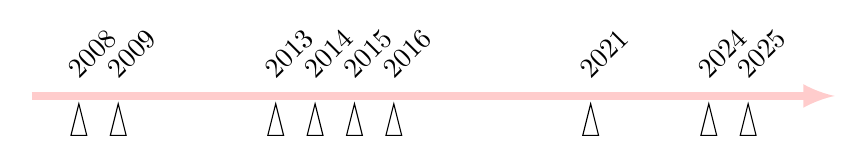
\begin{tikzpicture}[xscale=0.5]%[scale=0.9, every node/.style={scale=0.6}]
    % \draw[line width=2mm,-latex,red!20] (-0.2,0) -- (9,0);
    \draw[line width=1mm,-latex,red!20] (-0.2,0) -- (20+0.2,0);
    \foreach \X [evaluate=\X as \Y using int(\X-2007),count=\Z] in {2008,2009,2013,2014,2015,2016,2021,2024,2025}
    {
      \draw[highlight on=<\Z>] ({\Y-0.2},-0.5) -- ({\Y+0.2},-0.5) -- (\Y,-0.1) -- cycle;
      \node[anchor=south,highlight on=<\Z>,fill=white,rotate=45,anchor=south
      west,inner sep=0pt] at (\Y,0.2) {\X};
    }
  \end{tikzpicture}

  \begin{itemize}[<+->]
    \item<1> 2008: Chrome is first released on Windows
    \item<2> 2009: Apple publishes HLS spec
    \item<3> 2013: Chrome launches MSE (the basis for ShakaPlayer, HLS.js, \& others)
    \item<4> 2014: ShakaPlayer is created % December 19th
    \item<5> 2015: HLS.js is created % January 30th
    \item<6> 2016: Chrome on Android supports HLS
    \item<7> 2021: HLS in Chrome work starts
    \item<8> 2024: New HLS player on Chrome for Android
    \item<9> 2025: Chrome supports HLS on desktop
  \end{itemize}
\end{frame}

\iffalse
\begin{frame}
  \frametitle{What's actually in scope?}
  \begin{itemize}[<+->]
    \item<1> Test
  \end{itemize}
\end{frame}

\begin{frame}
  \frametitle{Questions I know you'll all have}
  \begin{itemize}[<+->]
    \item<1> Isn't MSE Good enough?
    \item<2> Why not embed an existing player?
    \item<3> What about DASH?
  \end{itemize}
\end{frame}
\fi

\begin{frame}
  \frametitle{Why did you subtitle this talk with a mini rant about robustness anyway?}
  \begin{itemize}[<+->]
    \item<1-2> The Robustness Principle
    \begin{itemize}[<+->]
      \item<2> "Be conservative in what you send, be liberal in what you accept"
      %\item<2> https://datatracker.ietf.org/doc/html/rfc761#section-2.10
    \end{itemize}
    \item<3> What good is a spec when nobody follows it?
  \end{itemize}
\end{frame}

\begin{frame}
  \frametitle{HLS Quirks}
  \begin{itemize}[<+->]
    \item<1-3> A "Clean Room" lexer \& parser
      \begin{itemize}[<+->]
        \item<2-3> Some of us like doing this you know...
        \item<3-3> Entirely C++
      \end{itemize}
    \item<4-6> A greatly-delayed launch
      \begin{itemize}[<+->]
        \item<5-6> Telemetry :'(
        \item<6-6> An extra 6 months
      \end{itemize}
    \item<7> Parser Quirks (media/formats/hls/quirks.h)
      \begin{itemize}[<+->]
        \item<7> https://cs.chromium.org
      \end{itemize}
    \item<8-9> A plea to the community
      \begin{itemize}[<+->]
        \item<8-9> HLS content generators: Please stick to spec!
        \item<9-9> HLS players: Reject malformatted manifests!
      \end{itemize}
  \end{itemize}
\end{frame}

\end{document}